\section{Resultados}\label{sec:resultados}

Los resultados se presentan siguiendo las dos etapas del estudio sobre las predicciones OOF primarias ($28$ configuraciones, $14\,625$ unidades por variante, cero errores): el desempeño frente a las $22$ referencias oficiales en energía bruta, y su reconciliación inferencial y en factor de capacidad adimensional, junto con los estudios diagnósticos en $D+1$.

\subsection{Desempeño global en las 28 configuraciones y comparación Fixed vs.\ HPO}

Sobre el soporte común alineado con los $22$ modelos de referencia en energía bruta ($\text{kWh}$), \texttt{SM-CFHR-Fixed} ($B=0$) alcanza un rango ordinal medio de $\mathbf{2{,}93/23}$ en $\mathrm{MAE}_{\mathrm{macro}}$ ($\text{kWh}$), obtiene $\mathbf{18/28}$ victorias descriptivas frente al mejor competidor de biblioteca (\texttt{Mejor\_Bib}, $10/28$ derrotas), $\mathbf{22/28}$ frente al mejor modelo residual (\textit{custom}) y $\mathbf{15/28}$ frente a \texttt{MM30} (Tabla~\ref{tab:res_familias}). Por régimen y familia, el desempeño es marcadamente asimétrico:
\begin{itemize}
    \item \textbf{Horizonte $D+1$ y generalización espaciotemporal (ET):} en $D+1$ ET con cinco variables logra rango $1/23$ con reducción de $-22{,}16\%$ frente a \texttt{Mejor\_Bib} ($59\,803{,}6$ frente a $76\,831{,}1$~kWh/día, $\mathrm{Skill}=28{,}80\%$ sobre \texttt{MM30}). En $D+1$ intraplanta con clima obtiene $61\,297{,}1$~kWh/día (rango $12/23$, $-0{,}22\%$ frente a biblioteca).
    \item \textbf{Esquema recursivo sin clima ($7$--$28$~días):} mantiene rango medio $2{,}00/23$ en ET ($4/4$ victorias sobre biblioteca, $-1{,}70\%$ medio) y $1{,}50/23$ en intraplanta ($3/4$ victorias sobre biblioteca, $-0{,}27\%$ medio), aunque por debajo de \texttt{MM30} en ET.
    \item \textbf{Esquema directo acumulado sin clima ($7$--$28$~días):} es competitivo en ET ($3/4$ victorias frente a biblioteca, rango medio $3{,}25/23$, $-1{,}63\%$ medio), pero se degrada sistemáticamente en intraplanta ($1/4$ victorias, $+13{,}27\%$ medio, alcanzando $+24{,}24\%$ en $H=28$~días frente a \texttt{k-NN}).
    \item \textbf{Acoplamiento con NOAA GEFSv12 ($7$--$28$~días):} en ET alcanza rango $\mathbf{1{,}00/23}$ en los cuatro horizontes ($4/4$ victorias frente a biblioteca y \texttt{MM30}, $-11{,}84\%$ medio frente a biblioteca); en intraplanta obtiene rango medio $2{,}00/23$ ($0/4$ frente a biblioteca, $+1{,}04\%$, pero $4/4$ sobre \texttt{MM30}).
\end{itemize}

\begin{table}[!htbp]
\caption{Resumen comparativo por familia de escenarios de \texttt{SM-CFHR-Fixed} ($B=0$) sobre el soporte común alineado ($28$ escenarios, $23$ modelos en $\text{kWh}$).}\label{tab:res_familias}
\centering
\scriptsize
\begin{tabular}{llccccc}
\toprule
Familia & Tarea & Esc. & Rango medio & Vic.\ vs.\ Bib. & Vic.\ vs.\ MM30 & $\Delta$ medio vs.\ Bib. (\%) \\
\midrule
$D+1$ & Espaciotemporal & $2$ & $1{,}00$ & $2/2$ & $2/2$ & $-11{,}30\%$ \\
$D+1$ & Intraplanta & $2$ & $7{,}50$ & $1/2$ & $2/2$ & $+0{,}07\%$ \\
Directo sin clima & Espaciotemporal & $4$ & $3{,}25$ & $3/4$ & $0/4$ & $-1{,}63\%$ \\
Directo sin clima & Intraplanta & $4$ & $6{,}50$ & $1/4$ & $0/4$ & $+13{,}27\%$ \\
Rec.\ sin clima & Espaciotemporal & $4$ & $2{,}00$ & $4/4$ & $0/4$ & $-1{,}70\%$ \\
Rec.\ sin clima & Intraplanta & $4$ & $1{,}50$ & $3/4$ & $3/4$ & $-0{,}27\%$ \\
Rec.\ + GEFSv12 & Espaciotemporal & $4$ & $1{,}00$ & $4/4$ & $4/4$ & $-11{,}84\%$ \\
Rec.\ + GEFSv12 & Intraplanta & $4$ & $2{,}00$ & $0/4$ & $4/4$ & $+1{,}04\%$ \\
\bottomrule
\end{tabular}
\end{table}

Al comparar directamente ambas variantes mediante $\mathrm{MAE}_{\mathrm{macro}}$, \texttt{SM-CFHR-HPO} ($B=25$, $14\,552$ estudios Optuna con $25$ ensayos válidos y $73$ unidades sin historial suficiente) solo mejora a \texttt{SM-CFHR-Fixed} ($B=0$) en $\mathbf{9/28}$ escenarios ---todos intraplanta---, mientras \texttt{Fixed} vence en $14/14$ escenarios espaciotemporales y $5/14$ intraplanta ($19/28$ en total; rango medio $2{,}93$ frente a $3{,}86/23$), con un coste de pared $59\times$ menor (Figura~\ref{fig:res_oof_rankings}).

\begin{figure}[!htbp]
\centering
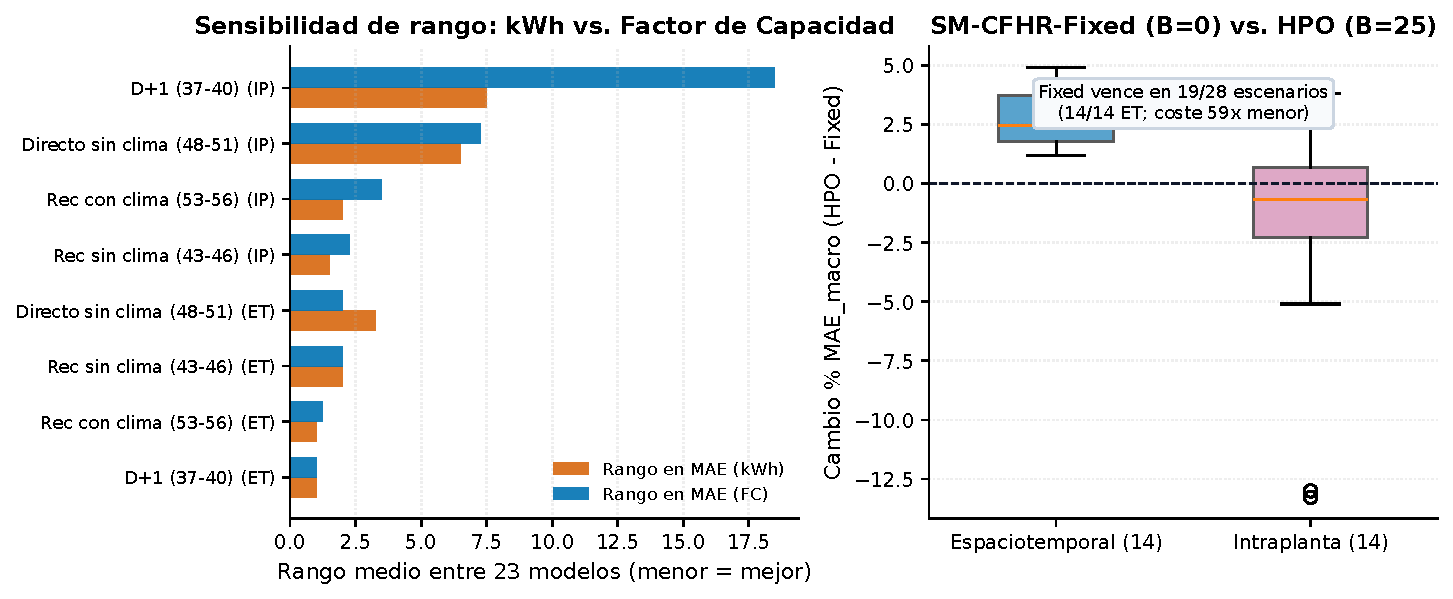
\includegraphics[width=0.98\textwidth]{figures/fig_res_oof_rankings_y_fixed_hpo.pdf}
\caption{Evaluación OOF primaria y métricas adimensionales: sensibilidad del rango medio entre $\text{kWh}$ ($2{,}93/23$) y factor de capacidad ($4{,}00/23$), y comparación pareada entre \texttt{SM-CFHR-Fixed} ($B=0$) y \texttt{SM-CFHR-HPO} ($B=25$).}
\label{fig:res_oof_rankings}
\end{figure}

\subsection{Protocolo original (v1.0.3), análisis retrospectivo (v2.0.0) y métricas en factor de capacidad}

Bajo el protocolo original congelado \texttt{v1.0.3} ($T_{\mathrm{eff}} \ge 2H$ sobre promedios simples por origen), únicamente $2/15$ contrastes DM--HLN--HAC frente a \texttt{Mejor\_Bib} alcanzaban significancia tras Holm ($D+1$ ET con clima y \texttt{RecGEFSv12} ET $7$d), excluyendo $13$ escenarios de horizontes largos. En la adaptación inferencial retrospectiva \texttt{v2.0.0} sobre los $28$ escenarios completos a partir de las mismas predicciones OOF guardadas sin reentrenar:
\begin{enumerate}
    \item \textbf{Inversiones de signo entre $\mathrm{MAE}_{\mathrm{macro}}$ y promedio por origen:} el desbalance de disponibilidad entre plantas ($1$ a $17$ centrales por origen) invertía el signo de $\Delta\mathrm{MAE}$ en $4/28$ escenarios (\texttt{D1\_IP\_sin\_clima}, \texttt{RecSinClima\_IP\_14d}, \texttt{RecSinClima\_IP\_28d} y \texttt{DirectoSinClima\_IP\_7d}), ninguno significativo ($p \ge 0{,}28$).
    \item \textbf{DM--HLN--HAC y bootstrap sincronizado sobre $\mathrm{MAE}_{\mathrm{macro}}$ (análisis retrospectivo):} con $h_{\mathrm{serie}}=1$ en bloques disjuntos y serie macro-alineada $z_t^{\mathrm{macro}}$, todos los $5/5$ escenarios \texttt{ET + Clima} ($D+1$ y $7$, $14$, $21$, $28$~días) muestran diferencias estadísticamente significativas tras Holm por familia frente a \texttt{Mejor\_Bib} seleccionado \textit{ex post} ($p_{\mathrm{Holm}} \le 5{,}21\times 10^{-6}$), manteniendo $0$ diferencias significativas en régimen intraplanta o sin clima. Debe destacarse como cautela muestral que en \texttt{RecGEFSv12 ET} de $21$ y $28$ días los tamaños efectivos se sitúan cerca del umbral descriptivo de $30$ ($T_{\mathrm{eff,macro}} = 31{,}35$ y $30{,}82$, respectivamente) con solo $G=7$ zonas espaciales. Frente a referencias preespecificadas en el diseño, \texttt{SM-CFHR-Fixed} obtiene $7/28$ diferencias favorables significativas ($0$ desfavorables) frente a \texttt{MM30} y $4/28$ frente a \texttt{SM-CFHR-HPO} ($1/28$ desfavorable).
    \item \textbf{Análisis secundario retrospectivo frente a las $9$ bibliotecas ($252$ contrastes):} en el archivo de reconciliación \texttt{v2.0.0} sobre el universo global de $252$ comparaciones ($9$ bibliotecas $\times$ $28$ escenarios), todas las $45/45$ comparaciones pareadas en los cinco escenarios \texttt{ET + Clima} presentan diferencia macro favorable ($\Delta\mathrm{MAE}_{\mathrm{macro}} < 0$) y resultan significativas bajo Holm global ($p_{\mathrm{Holm,252}} < 0{,}05$, con máximos por escenario de $9{,}03\times 10^{-22}$ en $D+1$, $1{,}41\times 10^{-9}$ en $7$d, $1{,}34\times 10^{-5}$ en $14$d, $3{,}58\times 10^{-3}$ en $21$d y $4{,}17\times 10^{-2}$ en $28$d). Este resultado proviene de un análisis exploratorio retrospectivo sobre la cohorte ya estudiada y no constituye una validación prospectiva independiente.
    \item \textbf{SPA y MCS ($B=5\,000$):} en \texttt{MCS} ($T_{\max}$ unilateral) sobre $\mathrm{MAE}_{\mathrm{macro}}$, \texttt{SM-CFHR-Fixed} sobrevive en $27/28$ escenarios del universo completo y como único superviviente ($1/10$) en $7/28$ entre bibliotecas (Material Suplementario, Sección~S4).
    \item \textbf{Métricas reales en factor de capacidad ($\mathrm{MAE}_{\mathrm{CF,macro}}$):} al normalizar cada observación por $24\,000\,C_{i,t}$ vigente (incluidas las $6$ centrales con ampliaciones escalonadas), el peso de las plantas mayores (como \texttt{GYPO}, $370$--$388$~MW) deja de dominar la media. El rango medio de \texttt{SM-CFHR-Fixed} pasa de $2{,}93/23$ ($\text{kWh}$) a $\mathbf{4{,}00/23}$ (CF), y las victorias descriptivas frente a \texttt{Mejor\_Bib} de $18/28$ a $16/28$.
\end{enumerate}

Las Figuras~\ref{fig:res_oof_planta}, \ref{fig:res_oof_d1}, \ref{fig:res_oof_rec} y \ref{fig:res_oof_dir} ilustran el desempeño por planta y grupo espacial (con capacidad diaria causal al origen y soporte pareado) junto con trayectorias ilustrativas en $D+1$, recursivo multihorizonte y directo acumulado.

\begin{figure}[!htbp]
\centering
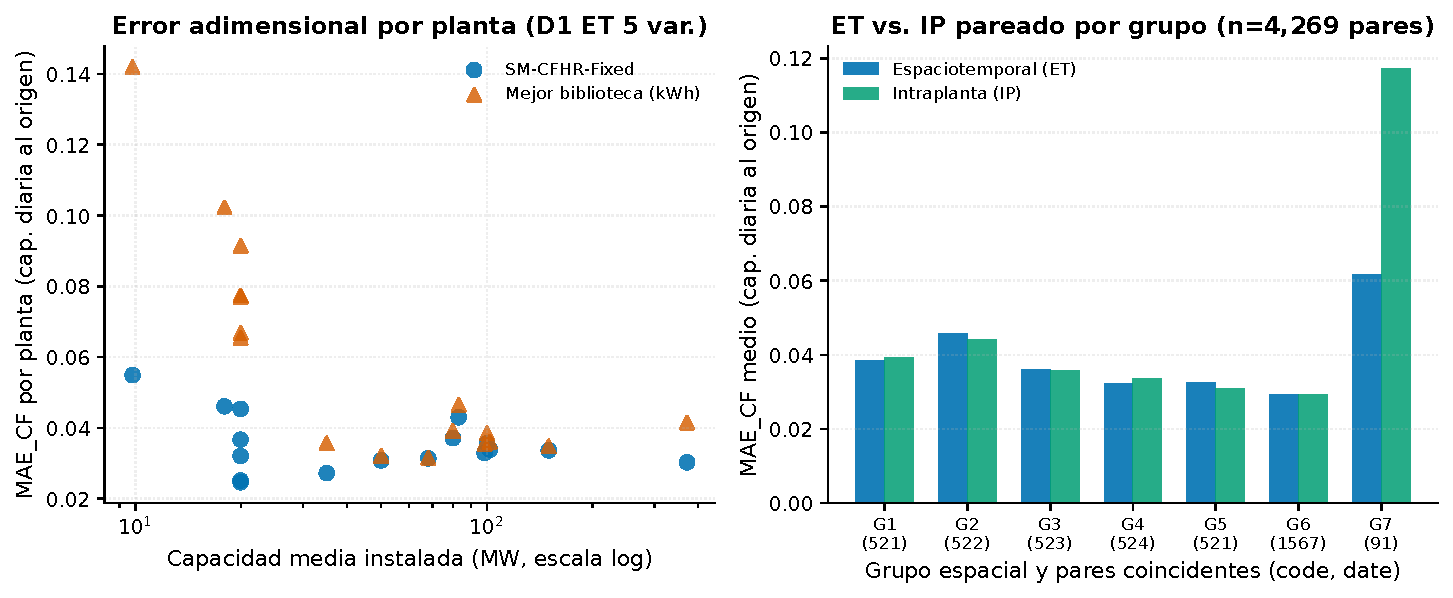
\includegraphics[width=0.98\textwidth]{figures/fig_res_oof_planta_y_grupos.pdf}
\caption{Error adimensional $\mathrm{MAE}_{\mathrm{CF}}$ por planta (normalizado observación por observación con la capacidad diaria al origen) frente a la capacidad media en \texttt{D1\_ET\_5var} (izquierda) y comparación ET frente a IP estrictamente pareada por \texttt{(code, date)} en los $7$ grupos espaciales ($n=4\,269$ pares coincidentes; grupo~7 con $n=91$ pares frente a $134$ en ET sin parear; derecha).}
\label{fig:res_oof_planta}
\end{figure}

\begin{figure}[!htbp]
\centering
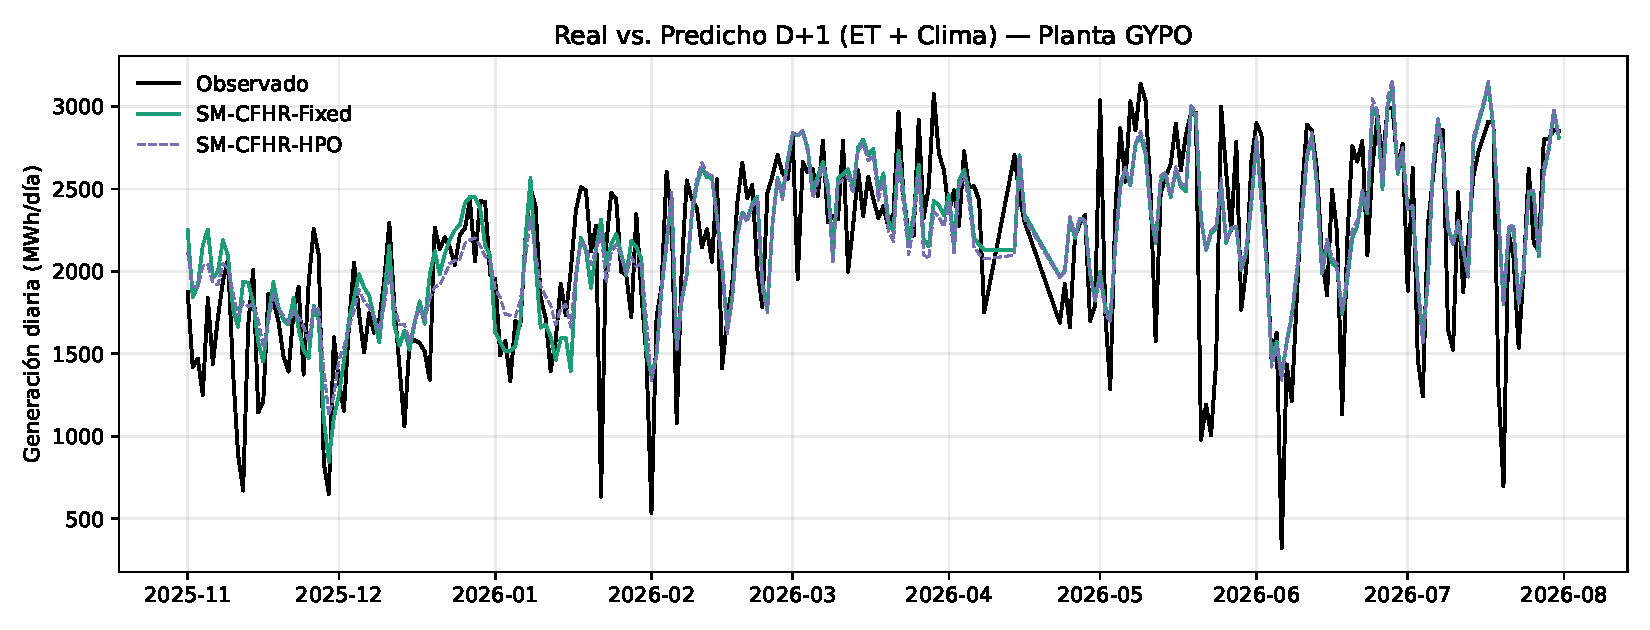
\includegraphics[width=0.95\textwidth]{figures/fig_res_oof_real_vs_pred_d1.pdf}
\caption{Ejemplo ilustrativo de generación diaria real frente a predicha en $D+1$ (\texttt{D1\_ET\_5var}, noviembre de $2025$ a julio de $2026$) para la central \texttt{GYPO}, seleccionada por registrar la mayor generación media y capacidad instalada de la cohorte ($370$--$388$~MW).}
\label{fig:res_oof_d1}
\end{figure}

\begin{figure}[!htbp]
\centering
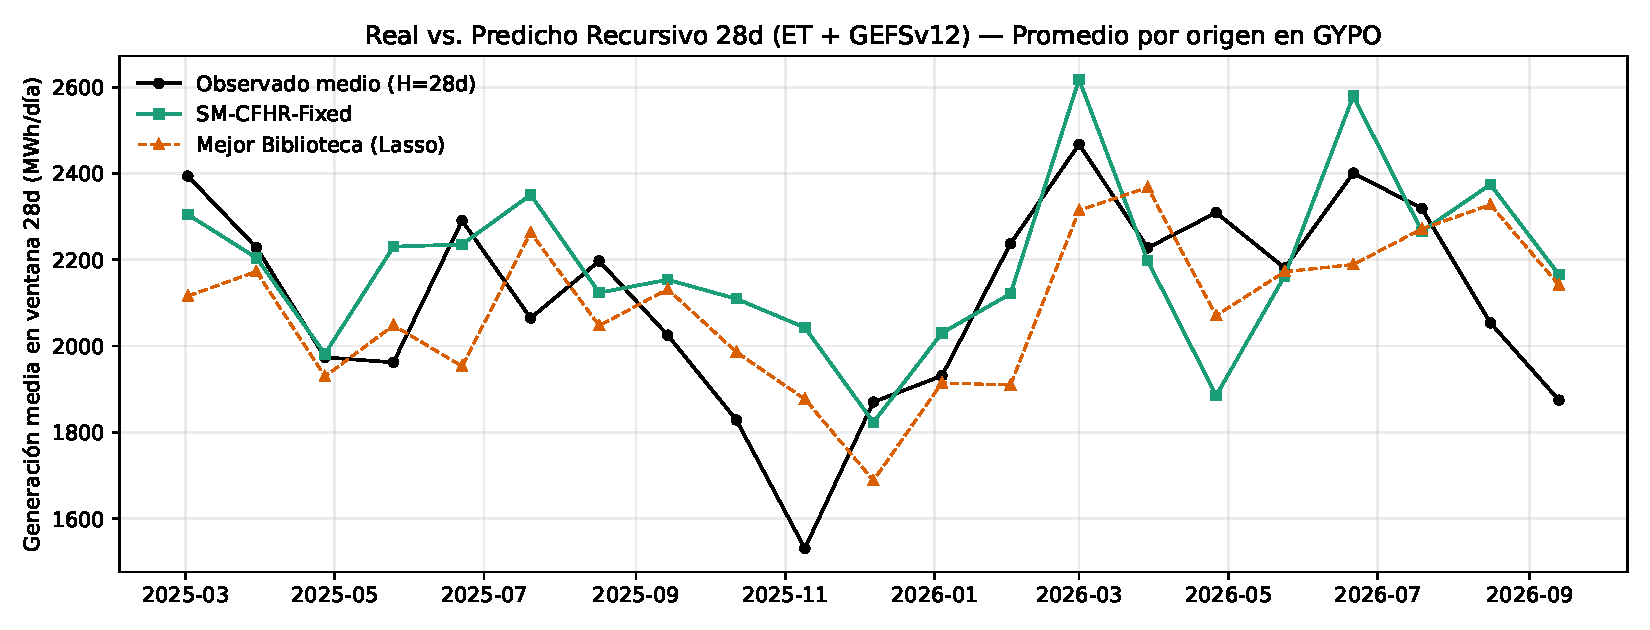
\includegraphics[width=0.95\textwidth]{figures/fig_res_oof_real_vs_pred_rec.pdf}
\caption{Ejemplo ilustrativo de trayectorias promedio por origen ($H=28$~días) reales frente a predichas en el esquema recursivo con meteorología GEFSv12 (\texttt{RecGEFSv12\_ET\_28d}, marzo de $2025$ a septiembre de $2026$) para la central \texttt{GYPO} (mayor generación media de la cohorte).}
\label{fig:res_oof_rec}
\end{figure}

\begin{figure}[!htbp]
\centering
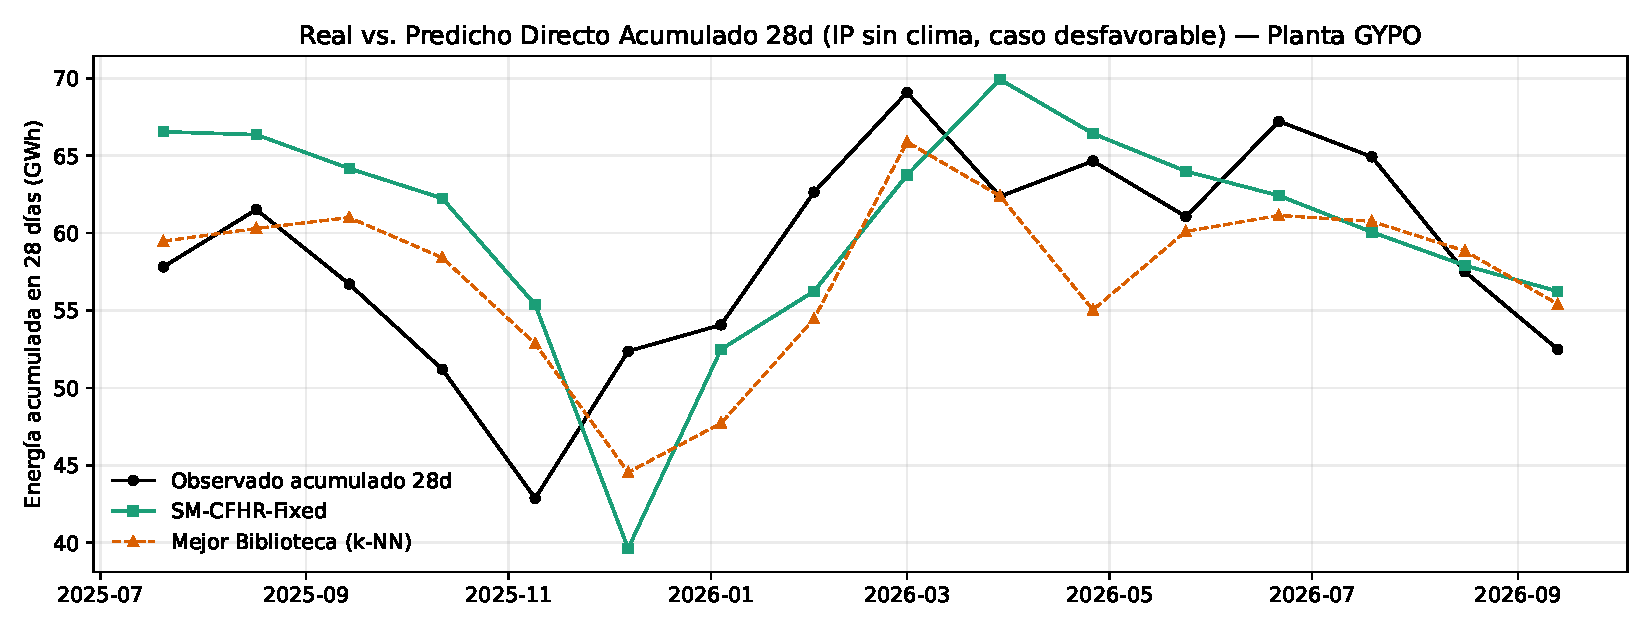
\includegraphics[width=0.95\textwidth]{figures/fig_res_oof_real_vs_pred_dir.pdf}
\caption{Ejemplo ilustrativo de energía acumulada en ventanas de $28$~días observada frente a predicha en el esquema directo sin meteorología (\texttt{DirectoSinClima\_IP\_28d}, caso desfavorable) para la central \texttt{GYPO} (seleccionada por mayor generación media de la cohorte, no como muestra aleatoria).}
\label{fig:res_oof_dir}
\end{figure}

\subsection{Estudios diagnósticos en $D+1$: ablación, estrés, incertidumbre e interpretabilidad}

Sobre el panel real $D+1$ con corte cronológico estricto ($\max t_{\mathrm{train}} < \min t_{\mathrm{val}}$) se observan los siguientes resultados (Tabla~\ref{tab:res_ablaciones} y Figura~\ref{fig:res_oof_ablaciones}):
\begin{enumerate}
    \item \textbf{Ablación controlada en $D+1$:} suprimir la normalización por factor de capacidad (\texttt{energia\_bruta\_vs\_cf}) multiplica el error por $4{,}45\times$ ($270\,035{,}5$ frente a $60\,631{,}2$~kWh/día; $0{,}23065$ frente a $0{,}03488$ CF). La pérdida de Huber mejora marginalmente sobre $L_2$ en datos limpios ($60\,631{,}2$ frente a $60\,784{,}0$~kWh/día), mientras \texttt{sin\_monotonia} y \texttt{escala\_std\_vs\_mad} coinciden con el modelo completo en este corte porque los pesos naturales de \texttt{cf30} ($+0{,}4591$) y \texttt{rad\_pron} ($+0{,}0863$) ya resultaron positivos.
    \item \textbf{Semillas y estrés sintético en $D+1$:} \texttt{SM-CFHR-Fixed} es determinista en las $10$ semillas ($56\,437{,}8$~kWh/día constantes), frente a la variabilidad de \texttt{HPO} ($55\,660{,}9$--$59\,124{,}8$~kWh/día). Bajo contaminación del $5\%$ y $10\%$ de atípicos en entrenamiento, Huber mantiene estable el error en validación limpia ($0{,}03488 \to 0{,}03491$ CF) mientras $L_2$ se degrada ($0{,}03496 \to 0{,}03749$ CF).
    \item \textbf{Incertidumbre conforme temporal e interpretabilidad:} sobre $n_{\mathrm{cal}}=1\,720$ residuos pasados, los intervalos conformes alcanzan coberturas empíricas de $83{,}24\%$ (para $90\%$ nominal, semiancho $0{,}0662$ CF) y $69{,}25\%$ (para $80\%$ nominal, semiancho $0{,}0480$ CF), reflejando deriva temporal entre bloques. En interpretabilidad aditiva exacta, los predictores dominantes son \texttt{cf30} ($0{,}0255$ CF), \texttt{anom\_rad} ($0{,}0107$) y \texttt{anom\_nube} ($0{,}0107$).
\end{enumerate}

\begin{table}[!htbp]
\caption{Estudio diagnóstico de ablación controlada sobre el panel real $D+1$ con corte cronológico estricto.}\label{tab:res_ablaciones}
\centering
\scriptsize
\begin{tabular}{lcc}
\toprule
Variante de ablación & $\mathrm{MAE}_{\mathrm{CF}}$ & $\mathrm{MAE}_{\mathrm{kWh/d\acute{\imath}a}}$ \\
\midrule
\texttt{SM-CFHR\_completo} & $0{,}03488$ & $60\,631{,}2$ \\
\texttt{sin\_l2\_estructurada} & $0{,}03487$ & $60\,606{,}3$ \\
\texttt{sin\_monotonia} & $0{,}03488$ & $60\,631{,}2$ \\
\texttt{escala\_std\_vs\_mad} & $0{,}03488$ & $60\,631{,}2$ \\
\texttt{sin\_huber\_L2} & $0{,}03496$ & $60\,784{,}0$ \\
\texttt{energia\_bruta\_vs\_cf} & $0{,}23065$ & $270\,035{,}5$ \\
\bottomrule
\end{tabular}
\end{table}

\begin{figure}[!htbp]
\centering
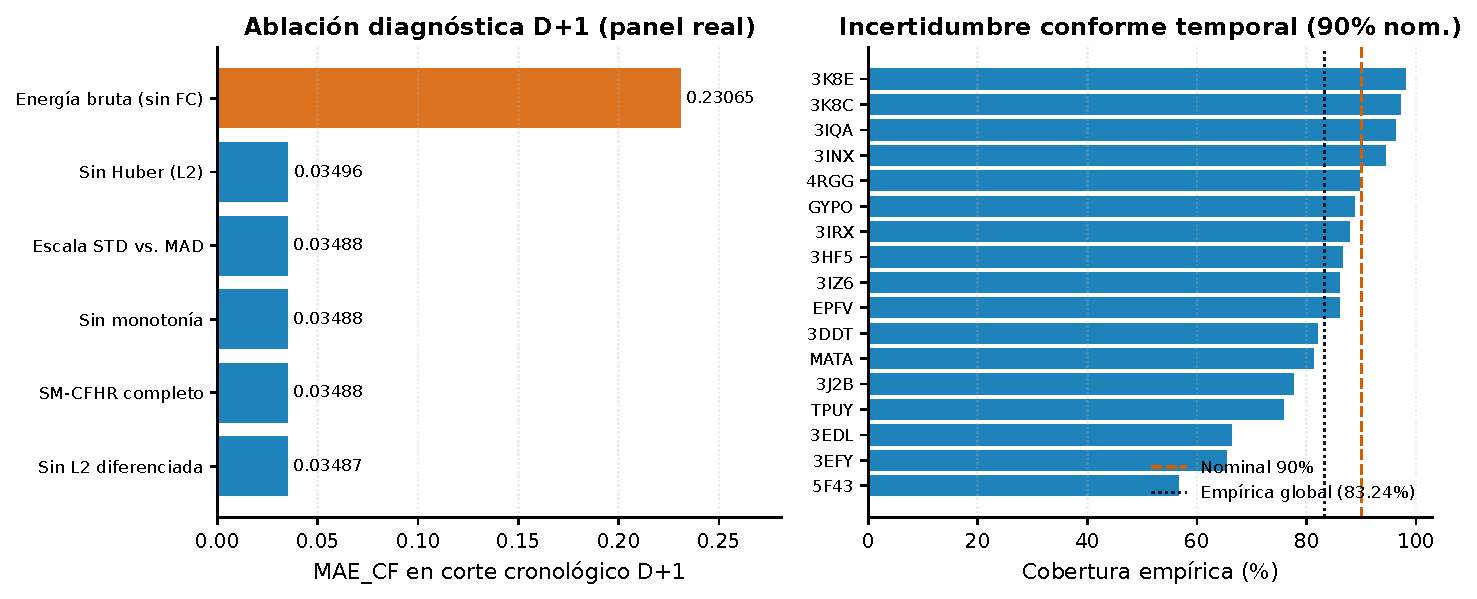
\includegraphics[width=0.98\textwidth]{figures/fig_res_oof_ablaciones_y_conformal.pdf}
\caption{Ablación diagnóstica en $D+1$ (izquierda) y cobertura empírica por central de los intervalos conformes temporales al $90\%$ nominal (derecha).}
\label{fig:res_oof_ablaciones}
\end{figure}

\subsection{Síntesis de hipótesis científicas H1--H4}

\begin{table}[!htbp]
\caption{Estado verificado de las hipótesis H1--H4 sobre las predicciones OOF congeladas y su reconciliación inferencial.}\label{tab:res_hipotesis}
\scriptsize
\setlength{\tabcolsep}{3.5pt}
\begin{tabular}{@{}p{2.3cm}p{2.7cm}p{6.5cm}@{}}
\toprule
Hipótesis & Estado verificado & Evidencia cuantitativa exacta \\
\midrule
\textbf{H1} (Normalización FC en ET) & \textbf{Respaldada solo en comparación de sistemas frente a referencias en $\text{kWh}$ (no aislada)} & En $D+1$ ET con clima logra rango $1/23$ ($-22{,}16\%$ frente a \texttt{Mejor\_Bib} en $\text{kWh}$) y en el corte único $D+1$ retirar FC multiplica el error por $4{,}45\times$; dado que las $22$ referencias operaron en energía bruta, la evidencia cerrada no aísla causalmente la normalización frente al estimador. \\
\textbf{H2} (Diferencias pareadas retrospectivas) & \textbf{Acotada a ET + Clima}; rechazada como superioridad universal & En \texttt{v1.0.3} ($T_{\mathrm{eff}} \ge 2H$): $2/15$ significativas; en el análisis retrospectivo \texttt{v2.0.0} sobre $\mathrm{MAE}_{\mathrm{macro}}$: $5/5$ en \texttt{ET + Clima} frente a \texttt{Mejor\_Bib} ($p_{\mathrm{Holm}} \le 5{,}21\times 10^{-6}$) y $45/45$ en el universo global de $252$ contrastes frente a bibliotecas ($p_{\mathrm{Holm,252}} \le 0{,}0417$), con $0$ en IP o sin clima y derrotas hasta $+24{,}24\%$ en \texttt{DirectoSinClima\_IP}. \\
\textbf{H3} (Componentes estructurales en $D+1$) & \textbf{Parcial / dependiente del corte} & La normalización FC explica la mayor caída ($4{,}45\times$); Huber aporta estabilidad bajo contaminación sintética ($10\%$); monotonía y MAD coinciden con el corte limpio sin restricción. \\
\textbf{H4} (Fixed vs.\ HPO) & \textbf{Refutada para HPO}; \texttt{Fixed} domina en precisión y coste & \texttt{Fixed} ($B=0$) supera a \texttt{HPO} ($B=25$) en $19/28$ escenarios ($14/14$ ET; $4$ victorias Holm frente a $1$ derrota) con coste $59\times$ menor. \\
\bottomrule
\end{tabular}
\end{table}
